\section{Overfitting a regularizace}\label{sec:preuceni}

Sekce~\ref{sec:evaluace} ukázala, \emph{jak} chybu modelu poctivě měřit. Tato sekce vysvětluje, \emph{proč} se trénovací a~generalizační chyba rozcházejí: model může být na úlohu příliš slabý (\emph{underfitting}, podučení) nebo příliš silný a~zapamatovat si i~šum (\emph{overfitting}, přeučení). Zavedeme \emph{kapacitu modelu} jako škálu mezi těmito extrémy, ukážeme, jak ji ovládat \emph{regularizací} ($L^2$, $L^1$) a~\emph{early stopping}, a~na závěr rozebereme \emph{prokletí dimenzionality} -- proč je vysoká dimenze příznaků sama o~sobě zdrojem overfittingu.

\begin{poznamka}[Vztah k~S1]
Okruh S1 zmiňuje overfitting jen v~souvislosti s~\emph{Ockhamovou břitvou} (preferuj nejjednodušší hypotézu konzistentní s~daty). Zde to rozvádíme do hloubky, kterou S1 výslovně přenechává S3: kapacita modelu, generalizační chyba, regularizační techniky a~prokletí dimenzionality. Konkrétní aplikace $L^2$ na lineární regresi je v~sekci~\ref{sec:linreg}.
\end{poznamka}

\subsection{Generalizační chyba, underfitting a overfitting}

\begin{definice}[Trénovací a~generalizační chyba]
\textbf{Trénovací chyba} je chyba modelu na trénovací množině, na které se učil. \textbf{Generalizační chyba} (chyba zobecnění, též \emph{testovací chyba}) je \emph{očekávaná} chyba na nových, neviděných příkladech ze stejného rozdělení generujícího data; odhadujeme ji chybou na nezávislé testovací množině (sekce~\ref{sec:evaluace}). Cílem učení je malá generalizační chyba, ne malá trénovací chyba.
\end{definice}

\begin{definice}[Underfitting a~overfitting]
\textbf{Underfitting} (podučení) nastane, když model nedokáže zachytit ani zákonitost v~trénovacích datech: trénovací \emph{i} generalizační chyba jsou velké. \textbf{Overfitting} (přeučení) nastane, když se model „naučí`` i~náhodný šum trénovací množiny: trénovací chyba je malá, ale generalizační chyba velká (mezera mezi nimi je velká).
\end{definice}

\begin{intuice}
Klasická ukázka je prokládání zašuměných bodů polynomem (obrázek níže). \emph{Přímka} (stupeň 1) je na sinusovku příliš tuhá -- nastává underfitting. Polynom \emph{vysokého stupně} (stupeň 9, deset koeficientů na $11$ bodů) projde body téměř přesně (trénovací chyba skoro nulová), ale mezi body divoce kmitá: zapamatoval si šum, ne tvar (overfitting). \emph{Střední stupeň} (zde 3) zachytí tvar a~šum ignoruje -- nejlépe generalizuje. Overfittovaný model je jako student, který nabiflováním odpoví na cvičné otázky doslova, ale u~nové otázky selže.
\end{intuice}

\begin{center}
\pgfplotsset{
  fitstyl/.style={width=5.3cm,height=4.4cm,
    xmin=-0.05,xmax=1.05,ymin=-1.7,ymax=1.7,
    xtick=\empty,ytick=\empty,axis lines=left,
    every axis plot/.append style={thick},
    title style={font=\small}},
}
\begin{tikzpicture}
\begin{axis}[fitstyl,title={underfitting (st.\ 1)}]
  \addplot[black!35,dashed] table[x=x,y=y]{src/fig/s2_poly_true.dat};
  \addplot[blue!60!black] table[x=x,y=y]{src/fig/s2_poly_deg1.dat};
  \addplot[only marks,mark=*,mark size=1.2pt,red!70!black] table[x=x,y=t]{src/fig/s2_poly_data.dat};
\end{axis}
\end{tikzpicture}\hfill
\begin{tikzpicture}
\begin{axis}[fitstyl,title={dobrý fit (st.\ 3)}]
  \addplot[black!35,dashed] table[x=x,y=y]{src/fig/s2_poly_true.dat};
  \addplot[green!45!black] table[x=x,y=y]{src/fig/s2_poly_deg3.dat};
  \addplot[only marks,mark=*,mark size=1.2pt,red!70!black] table[x=x,y=t]{src/fig/s2_poly_data.dat};
\end{axis}
\end{tikzpicture}\hfill
\begin{tikzpicture}
\begin{axis}[fitstyl,title={overfitting (st.\ 9)}]
  \addplot[black!35,dashed] table[x=x,y=y]{src/fig/s2_poly_true.dat};
  \addplot[red!60!black] table[x=x,y=y]{src/fig/s2_poly_deg9.dat};
  \addplot[only marks,mark=*,mark size=1.2pt,red!70!black] table[x=x,y=t]{src/fig/s2_poly_data.dat};
\end{axis}
\end{tikzpicture}
\obrpopis{Polynomy stupně 1, 3 a~9 proložené $11$~zašuměnými body (červeně) z~funkce $\sin(2\pi x)$ (čárkovaně pravá křivka). Trénovací RMSE klesá $0{,}56\to0{,}16\to0{,}01$: stupeň 1 nestačí (underfitting), stupeň 9 projde body téměř přesně, ale mimo ně kmitá (overfitting), stupeň 3 vystihne tvar nejlépe. Data vygenerována s~fixním seedem (\texttt{src/fig/gen\_s2\_polyfit.py}).}
\end{center}

\subsection{Kapacita modelu}

\begin{definice}[Kapacita modelu]
\textbf{Kapacita} modelu je neformálně jeho schopnost vyjádřit \emph{složité} funkce -- jak bohatá je třída funkcí, mezi nimiž učení vybírá. Rozlišujeme \emph{reprezentační kapacitu} (jaké funkce model vůbec umí vyjádřit, např.\ polynomy do stupně $M$) a~\emph{efektivní kapacitu} (kterých z~nich učící algoritmus reálně dosáhne, případně omezenou regularizací). U~polynomiální regrese roste kapacita se stupněm $M$; obecně s~počtem volných parametrů.
\end{definice}

\begin{intuice}
Kapacita je „regulátor`` mezi underfittingem a~overfittingem. \emph{Malá} kapacita $\Rightarrow$ underfitting (model je příliš tuhý). \emph{Velká} kapacita $\Rightarrow$ riziko overfittingu (model je tak ohebný, že se přizpůsobí i~šumu). Optimum je uprostřed. Kapacitu lze měnit nejen volbou modelu (stupeň polynomu, hloubka stromu, počet sousedů $k$), ale i~\emph{množstvím dat}: víc trénovacích příkladů relativní kapacitu snižuje (model už nemá dost volnosti zapamatovat si každý bod), takže více dat samo o~sobě overfitting tlumí.
\end{intuice}

\begin{center}
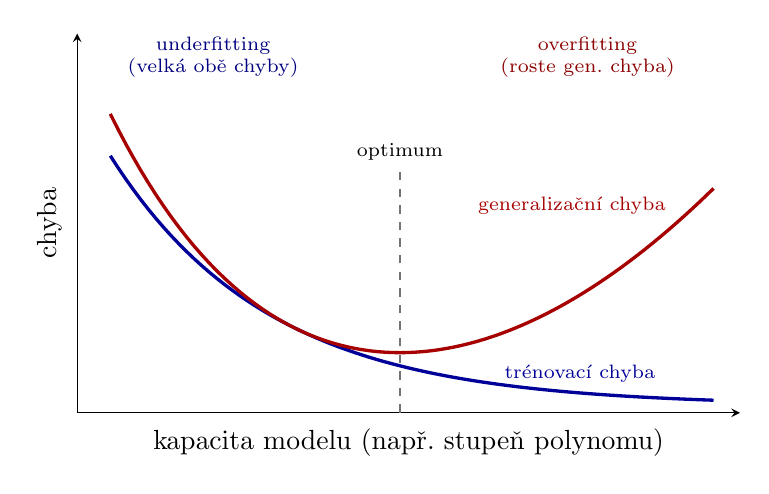
\begin{tikzpicture}
\begin{axis}[width=10.0cm,height=6.4cm,
  xlabel={kapacita modelu (např.\ stupeň polynomu)},ylabel={chyba},
  xmin=0,xmax=10,ymin=0,ymax=3.2,
  xtick=\empty,ytick=\empty,axis lines=left,clip=false,
  every axis plot/.append style={very thick}]
  % trénovací chyba: monotónně klesá
  \addplot[blue!60!black,domain=0.5:9.6,samples=80]{2.6*exp(0-0.42*x)+0.06};
  % generalizační chyba: U-tvar (klesá, pak roste)
  \addplot[red!65!black,domain=0.5:9.6,samples=80]{2.6*exp(0-0.42*x)+0.06+0.045*(x-3.3)^2};
  % optimum kapacity = minimum červené křivky (numericky x = 4,87)
  \draw[black!55,dashed] (axis cs:4.87,0) -- (axis cs:4.87,2.05);
  \node[font=\scriptsize,anchor=south] at (axis cs:4.87,2.05) {optimum};
  % oblasti
  \node[font=\scriptsize,blue!50!black,align=center] at (axis cs:2.05,3.0) {underfitting\\(velká obě chyby)};
  \node[font=\scriptsize,red!55!black,align=center] at (axis cs:7.7,3.0) {overfitting\\(roste gen.\ chyba)};
  % popisky křivek
  \node[font=\scriptsize,blue!60!black,anchor=west] at (axis cs:6.3,0.33) {trénovací chyba};
  \node[font=\scriptsize,red!65!black,anchor=west] at (axis cs:5.9,1.75) {generalizační chyba};
\end{axis}
\end{tikzpicture}
\obrpopis{Schematická závislost chyby na kapacitě modelu. Trénovací chyba (modře) s~rostoucí kapacitou monotónně klesá. Generalizační chyba (červeně) má tvar \emph{U}: nejdřív klesá (mizí underfitting), pak roste (model overfittuje). Optimální kapacita je v~minimu červené křivky; vlevo od něj je oblast underfittingu, vpravo overfittingu. Mezera mezi křivkami je míra overfittingu.}
\end{center}

\subsection{Regularizace}

\begin{definice}[Regularizace]
\textbf{Regularizace} je jakákoli úprava učícího algoritmu, jejímž záměrem je \emph{snížit generalizační chybu} (ne nutně trénovací). Typicky omezuje efektivní kapacitu modelu, takže ten musí dát přednost „jednodušším`` řešením a~hůře se přizpůsobí šumu.
\end{definice}

\begin{intuice}
Omezení kapacity zvenčí (menší stupeň polynomu) je hrubé -- skáče po celých číslech a~rovnou škrtá celé příznaky. Regularizace dovoluje \emph{plynule} škálovat, jak moc model „smí`` přizpůsobit váhy datům: necháme bohatou třídu funkcí, ale přidáme do ztrátové funkce \emph{trest za složitost}. Nejčastěji trestáme \emph{velikost vah} -- malé váhy znamenají hladší, méně rozkmitanou funkci.
\end{intuice}

\subsubsection*{$L^2$ a~$L^1$ regularizace}

\begin{definice}[$L^2$ a~$L^1$ regularizace]
K~původní ztrátové funkci $E_0(\mathbf{w})$ (např.\ součtu čtverců) přidáme penalizační člen úměrný normě vah:
\[
E_{L^2}(\mathbf{w}) = E_0(\mathbf{w}) + \frac{\lambda}{2}\,\|\mathbf{w}\|_2^2
  = E_0(\mathbf{w}) + \frac{\lambda}{2}\sum_{j} w_j^2,
\qquad
E_{L^1}(\mathbf{w}) = E_0(\mathbf{w}) + \lambda\,\|\mathbf{w}\|_1
  = E_0(\mathbf{w}) + \lambda\sum_{j} |w_j|.
\]
\textbf{$L^2$ regularizace} (též \emph{weight decay}, hřebenová / ridge regrese) trestá kvadrát eukleidovské normy; \textbf{$L^1$ regularizace} (lasso) trestá součet absolutních hodnot. \emph{Regularizační síla} $\lambda \ge 0$ je hyperparametr: $\lambda=0$ je bez regularizace, velké $\lambda$ tlačí váhy k~nule. Penalizace se obvykle \emph{nevztahuje na bias} $b$ (přes bias nelze overfittovat).
\end{definice}

\begin{intuice}[$L^2$ vyhlazuje, $L^1$ řídne]
Obě penalizace táhnou váhy k~nule, ale jinak. \textbf{$L^2$} zmenšuje \emph{všechny} váhy úměrně jejich velikosti -- velké srazí hodně, malé téměř nechá; vede k~mnoha \emph{malým, ale nenulovým} vahám, tedy k~hladkému modelu (gradient lineární predikce vůči vstupu jsou přímo váhy, $\nabla_{\mathbf{x}}\,\mathbf{w}^{\!\top}\mathbf{x}=\mathbf{w}$, takže malé váhy $=$ malé změny výstupu). \textbf{$L^1$} naopak tlačí část vah \emph{přesně na nulu} -- provádí tak \emph{výběr příznaků}: výsledný model je \emph{řídký} (sparse), používá jen podmnožinu příznaků. Proč rozdíl, ukazuje geometrie níže.
\end{intuice}

\begin{center}
\begin{tikzpicture}[scale=1.1]
% Geometrie ověřena numericky: střed elips W=(2,0.45), poloosy (1.4,1.0), osově zarovnané.
% Rostoucí kontura se DOTKNE jednotkového kruhu v (0.957,0.289) [mimo osy] (měřítko 0.762)
% a kosočtverce přesně v ROHU (1,0) [w2=0] (měřítko 0.844). Vykreslujeme dotykovou konturu
% jako vnější (obepíná celou oblast a dotýká se jen v bodě řešení).
\foreach \px/\title/\dia in {0/{$L^2$: dotyk mimo osy}/0, 6.6/{$L^1$: dotyk v~rohu}/1}{
  \begin{scope}[shift={(\px,0)}]
    \node[font=\small] at (0.6,2.35) {\title};
    \draw[osa] (-1.6,0) -- (3.2,0) node[below right=-1pt,font=\scriptsize]{$w_1$};
    \draw[osa] (0,-1.6) -- (0,2.1) node[right=1pt,font=\scriptsize]{$w_2$};
    \coordinate (W) at (2.0,0.45);
    \ifnum\dia=0
      % L2: kruh + kontury (vnější má měřítko 0.762, dotyk v (0.957,0.289))
      \foreach \s in {0.30,0.52,0.762}{ \draw[red!55!black] (W) ellipse ({1.4*\s} and {1.0*\s}); }
      \draw[blue!60!black,very thick,fill=blue!10,fill opacity=0.5] (0,0) circle (1.0);
      \fill[red!65!black] (W) circle (1.3pt);
      \node[font=\scriptsize,red!55!black,anchor=south west] at (2.05,0.5) {$\mathbf{w}^\star$};
      \coordinate (S) at (0.957,0.289);
      \fill[black] (S) circle (1.5pt);
      \node[font=\scriptsize,anchor=south west] at (1.0,0.34) {$\hat{\mathbf{w}}$};
      \node[font=\scriptsize,anchor=north,blue!55!black] at (0.0,-1.05) {obě složky $\neq 0$};
    \else
      % L1: kosočtverec + kontury (vnější má měřítko 0.844, dotyk v rohu (1,0))
      \foreach \s in {0.33,0.58,0.844}{ \draw[red!55!black] (W) ellipse ({1.4*\s} and {1.0*\s}); }
      \draw[blue!60!black,very thick,fill=blue!10,fill opacity=0.5]
        (1.0,0) -- (0,1.0) -- (-1.0,0) -- (0,-1.0) -- cycle;
      \fill[red!65!black] (W) circle (1.3pt);
      \node[font=\scriptsize,red!55!black,anchor=south west] at (2.05,0.5) {$\mathbf{w}^\star$};
      \coordinate (S) at (1.0,0);
      \fill[black] (S) circle (1.7pt);
      \node[font=\scriptsize,anchor=south west] at (1.06,0.07) {$\hat{\mathbf{w}}$};
      \node[font=\scriptsize,anchor=north,green!45!black] at (0.0,-1.05) {$w_2=0$ (řídké)};
    \fi
  \end{scope}
}
\end{tikzpicture}
\obrpopis{Geometrie regularizace. Červené elipsy jsou \emph{kontury} (vrstevnice) původní ztráty se středem v~nepenalizovaném optimu $\mathbf{w}^\star_{\text{MLE}}$ (maximum likelihood estimation, odhad maximální věrohodnosti). Regularizace nutí řešení $\hat{\mathbf{w}}$ dovnitř modré omezující oblasti; optimum leží tam, kde se nejmenší kontura oblasti \emph{dotkne}. Vlevo: \emph{$L^2$} oblast je kruh (hladký), dotyk nastane v~obecném bodě s~oběma složkami nenulovými. Vpravo: \emph{$L^1$} oblast je kosočtverec s~\emph{rohy} na osách; elipsa se ho typicky dotkne v~rohu, kde $w_2=0$ -- proto $L^1$ vynuluje váhy a~dává řídké řešení.}
\end{center}

\begin{poznamka}
$\lambda$ a~stupeň polynomu $M$ jsou \emph{hyperparametry} -- učící algoritmus je sám nenastaví, určujeme je zvenčí. Konkrétní dopad $L^2$ na uzavřené řešení lineární regrese (přechod $\mathbf{X}^{\!\top}\mathbf{X}\to\mathbf{X}^{\!\top}\mathbf{X}+\lambda\mathbf{I}$, vždy invertibilní) a~na krok SGD rozebíráme u~modelu, kde se to počítá -- v~sekci~\ref{sec:linreg}.
\end{poznamka}

\subsubsection*{Early stopping}

U~iterativně trénovaných modelů (gradientní sestup) lze kapacitu omezit i~\emph{časem}: čím déle trénujeme, tím víc se model přizpůsobuje datům včetně šumu.

\begin{definice}[Early stopping]
\textbf{Early stopping} (včasné zastavení) sleduje během trénování chybu na \emph{validační} množině a~trénink ukončí (resp.\ použije uložený model) ve chvíli, kdy validační chyba přestane klesat a~začne růst, i~když trénovací chyba dál klesá. Počet kroků (epoch) je tak vlastně hyperparametr laděný na validačních datech.
\end{definice}

\begin{intuice}
Trénovací chyba u~dostatečně kapacitního modelu klesá monotónně až k~nule, ale validační chyba má opět tvar \emph{U}: nejdřív klesá (model se učí zákonitost), pak roste (začíná se učit šum). Bod obratu je optimální okamžik zastavení -- model v~něm má nejlepší generalizaci. Early stopping je oblíbené, protože je levné (nevyžaduje volbu $\lambda$ ani opakované trénování) a~funguje jako forma regularizace: omezuje, jak daleko se váhy od počátku stačí pohnout. (Příbuznou technikou je \emph{dropout} u~neuronových sítí, mimo rozsah tohoto okruhu.)
\end{intuice}

\begin{center}
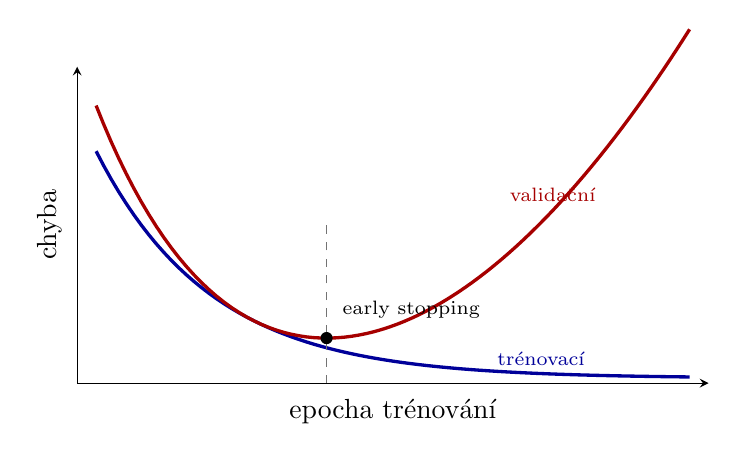
\begin{tikzpicture}
\begin{axis}[width=9.6cm,height=5.6cm,
  xlabel={epocha trénování},ylabel={chyba},
  xmin=0,xmax=10,ymin=0,ymax=2.6,
  xtick=\empty,ytick=\empty,axis lines=left,clip=false,
  every axis plot/.append style={very thick}]
  % trénovací chyba: klesá k nule
  \addplot[blue!60!black,domain=0.3:9.7,samples=80]{2.2*exp(0-0.55*x)+0.04};
  % validační chyba: U-tvar
  \addplot[red!65!black,domain=0.3:9.7,samples=80]{2.2*exp(0-0.55*x)+0.04+0.06*(x-2.8)^2};
  % bod early stopping = minimum validační křivky (numericky x = 3,95, y = 0,37)
  \draw[black!55,dashed] (axis cs:3.95,0) -- (axis cs:3.95,1.35);
  \fill[black] (axis cs:3.95,0.37) circle (2.2pt);
  \node[font=\scriptsize,anchor=south west] at (axis cs:4.05,0.45) {early stopping};
  \node[font=\scriptsize,blue!60!black,anchor=west] at (axis cs:6.5,0.2) {trénovací};
  \node[font=\scriptsize,red!65!black,anchor=west] at (axis cs:6.7,1.55) {validační};
\end{axis}
\end{tikzpicture}
\obrpopis{Early stopping. Trénovací chyba (modře) klesá k~nule, validační chyba (červeně) nejdřív klesá, pak roste -- model začíná overfittovat. V~minimu validační chyby (černá tečka) trénink zastavíme; další epochy už generalizaci jen zhoršují.}
\end{center}

\subsection{Prokletí dimenzionality}

\begin{definice}[Prokletí dimenzionality]
\textbf{Prokletí dimenzionality} (curse of dimensionality) je souhrn jevů, kvůli nimž se s~rostoucím počtem příznaků $D$ (dimenzí vstupu) učení dramaticky ztěžuje: objem prostoru roste exponenciálně, takže fixní množina dat je ve vysoké dimenzi \emph{řídká} (vzdálené, prázdné okolí každého bodu), a~vzdálenosti mezi body se vzájemně \emph{připodobňují}. K~pokrytí prostoru se stejnou hustotou bodů je třeba \emph{exponenciálně} mnoho příkladů v~$D$.
\end{definice}

\begin{intuice}
Tři tváře téhož jevu. \emph{(1)~Hustota:} $10$ bodů rovnoměrně pokryje úsečku $[0,1]$, ale $[0,1]^{10}$ jich vyžaduje $10^{10}$, aby byla mřížka stejně hustá -- jinak jsou data ve vysoké dimenzi téměř všude prázdná. \emph{(2)~Koncentrace objemu:} skoro celý objem vysokodimenzionální krychle (či koule) leží těsně u~povrchu, takže „typický`` bod je u~kraje, ne uvnitř. \emph{(3)~Koncentrace vzdáleností:} poměr nejbližšího a~nejvzdálenějšího souseda se blíží jedné, takže pojem „nejbližší soused`` ztrácí smysl -- to přímo dopadá na $k$-NN (sekce~\ref{sec:knn}). Důsledek pro učení: víc příznaků zvyšuje kapacitu, ale i~potřebu dat; nadbytečné příznaky proto raději odstraňujeme (výběr příznaků, $L^1$, PCA).
\end{intuice}

\begin{center}
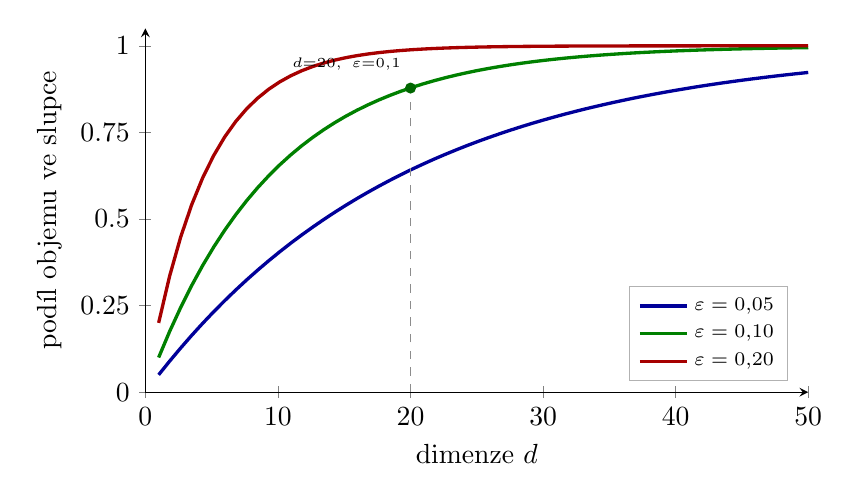
\begin{tikzpicture}
\begin{axis}[width=10.0cm,height=6.2cm,
  xlabel={dimenze $d$},ylabel={podíl objemu ve slupce},
  xmin=0,xmax=50,ymin=0,ymax=1.05,
  xtick={0,10,20,30,40,50},ytick={0,0.25,0.5,0.75,1},
  axis lines=left,clip=false,legend pos=south east,
  legend style={font=\scriptsize,draw=black!30},
  every axis plot/.append style={very thick}]
  \addplot[blue!60!black,domain=1:50,samples=60]{1-(1-0.05)^x};
  \addplot[green!50!black,domain=1:50,samples=60]{1-(1-0.1)^x};
  \addplot[red!65!black,domain=1:50,samples=60]{1-(1-0.2)^x};
  \legend{{$\varepsilon=0{,}05$},{$\varepsilon=0{,}10$},{$\varepsilon=0{,}20$}}
  \draw[black!45,dashed] (axis cs:20,0) -- (axis cs:20,0.878);
  \fill[green!40!black] (axis cs:20,0.878) circle (2pt);
  \node[font=\tiny,anchor=south east] at (axis cs:20,0.9) {$d{=}20,\ \varepsilon{=}0{,}1$};
\end{axis}
\end{tikzpicture}
\obrpopis{Koncentrace objemu: podíl objemu jednotkové krychle $[0,1]^d$, který leží ve vnější \emph{slupce} tloušťky $\varepsilon$ (mimo vnitřní krychli $[\varepsilon,1-\varepsilon]^d$), je $1-(1-2\varepsilon)^d$; zde kreslíme zjednodušeně podíl mimo zmenšenou krychli $[0,1-\varepsilon]^d$, tj.\ $1-(1-\varepsilon)^d$. Pro $\varepsilon=0{,}1$ a~$d=20$ vychází $1-0{,}9^{20}\approx0{,}878$, tj.\ skoro $88\,\%$ objemu je v~tenké slupce u~povrchu; pro $d=50$ je to $1-0{,}9^{50}\approx0{,}995$. Funkce je analytická, bez šumu.}
\end{center}

\begin{priklad}[Ilustrace: $L^1$ vynuluje váhu, $L^2$ ne]
\textbf{Zadání.} Mějme model se dvěma vahami, kde nepenalizované optimum ztráty je $\mathbf{w}^\star=(2,\,0{,}5)$ a~kontury ztráty jsou kružnice $\|\mathbf{w}-\mathbf{w}^\star\|^2=\text{konst.}$ (izotropní). Omezíme řešení podmínkou $\|\mathbf{w}\|\le 1$ ($L^2$), resp.\ $\|\mathbf{w}\|_1\le 1$ ($L^1$). Které řešení je řídké?

\smallskip
\textbf{Řešení.} Při \emph{kruhových} konturách je penalizované řešení průmět $\mathbf{w}^\star$ na omezující oblast (nejbližší bod oblasti k~$\mathbf{w}^\star$).
\emph{$L^2$ (kruh poloměru 1):} nejbližší bod je ve směru $\mathbf{w}^\star$, tj.\ $\hat{\mathbf{w}}=\mathbf{w}^\star/\|\mathbf{w}^\star\| = (2,\,0{,}5)/\sqrt{4{,}25}\approx(0{,}970,\,0{,}243)$ -- \emph{obě} složky nenulové.
\emph{$L^1$ (kosočtverec $|w_1|+|w_2|\le1$):} nejbližší bod ke vzdálenému $\mathbf{w}^\star=(2,\,0{,}5)$ je \emph{roh} $(1,\,0)$ (ověření: vzdálenost $\mathbf{w}^\star$ od $(1,0)$ je $\sqrt{1+0{,}25}\approx1{,}118$ a~každý jiný bod kosočtverce je dál), takže $\hat{\mathbf{w}}=(1,\,0)$ -- druhá váha je \emph{přesně nula}. $L^1$ tedy příznak $2$ vyřadil (řídké řešení), $L^2$ ho jen zmenšil. To je kvantitativní ukázka geometrie z~obrázku výše.
\end{priklad}

\begin{priklad}[SZZ podzim 2022 č.~18: L2 regularizace, porovnání modelů]
\szzotazka{podzim 2022}{18}{Přeučení a regularizace}\par
\textbf{Zadání.} Trénujeme lineární model pro regresi. (1)~Definujte střední čtvercovou chybu (MSE) a~upravenou chybovou funkci pro $L^2$ regularizaci. (2)~Dva lineární modely pro data se čtyřmi atributy,
\[
  M_1(\mathbf{x}) = x_1 - 2x_2 + 4x_3 - x_4 + 3, \qquad
  M_2(\mathbf{x}) = x_2 - 5x_3 + x_4 - 1,
\]
mají na daných datech \emph{stejnou} MSE. Který má menší hodnotu $L^2$-regularizované chyby? (3)~Uveďte alespoň jeden další způsob, jak zlepšit generalizaci.

\smallskip
\textbf{Řešení.} \emph{(1)} Střední čtvercová chyba je
\[
  \mathrm{MSE} = \frac{1}{n}\sum_{i=1}^{n} (y_i - \hat y_i)^2,
\]
kde $\hat y_i$ je predikce a~$y_i$ skutečná hodnota. Při $L^2$ regularizaci přidáme k~MSE penalizaci za velikost vah,
\[
  \mathrm{MSE} + \lambda \sum_{j} w_j^2,\qquad \lambda>0,
\]
přičemž absolutní člen (bias) se \emph{ne}regularizuje.

\emph{(2)} Regularizační člen závisí jen na vahách (bez biasu). Pro $M_1$ jsou váhy $(1,-2,4,-1)$, takže $\sum_j w_j^2 = 1+4+16+1 = \boxed{22}$; pro $M_2$ jsou váhy $(0,1,-5,1)$, takže $\sum_j w_j^2 = 0+1+25+1 = \boxed{27}$. Při stejné MSE má menší regularizovanou chybu model $\boldsymbol{M_1}$ ($22<27$).

\smallskip
\emph{Pozn.} Kdyby se regularizoval i~bias, vyšlo by $M_1$: $22+3^2=31$ a~$M_2$: $27+(-1)^2=28$, a~vyhrál by $M_2$. Právě proto je podstatné, že se bias neregularizuje.

\emph{(3)} Generalizaci lze zlepšit i~více trénovacími daty, výběrem/redukcí příznaků, předčasným zastavením (early stopping), dropoutem (u~neuronových sítí), kombinováním modelů (ensembling), $L^1$ regularizací nebo laděním hyperparametrů (např.\ $\lambda$) křížovou validací.
\end{priklad}
